% Neuroloop utilities - Library reference - Top level
% Written by Christopher Thomas.

\documentclass[letterpaper,11pt]{report}
\usepackage[letterpaper]{geometry}
\usepackage{graphicx}
\usepackage{verbatim}
\usepackage{placeins}
\usepackage{longtable}

\geometry{nohead,footskip=0.3in,margin=0.75in}

% Force my paragraph style, darnit.
\usepackage{indentfirst}
\setlength{\parskip}{\baselineskip}

% NOTE - "\thispagestyle" is used for part and chapter beginning pages, and
% overrides \pagestyle. Redefine it to be harmless.
% NOTE - The canonical solution ("\pagenumbering{gobble}") resets the page
% counter whenever it's used.
\renewcommand{\thispagestyle}[1]{}

% Custom macros.
\newcommand{\fixme}[1]{\textbf{FIXME: #1}}

\newcommand{\figdef}[3]
{\begin{figure}[htb]
\begin{center}#1\end{center}
\caption{#2}\label{#3}\end{figure}}

\newcommand{\tabdef}[3]
{\begin{table}[hb]
\begin{center}#1\end{center}
\caption{#2}\label{#3}\end{table}}

% Document body.
\begin{document}
%
% Title page.
%
\pagestyle{empty}

\begin{center}
%
\vspace*{1in}
{\Huge NeuroLoop Utilities -- Function Reference} \\
{\footnotesize Written by Christopher Thomas -- \today.}
%
\vspace*{1in}\\
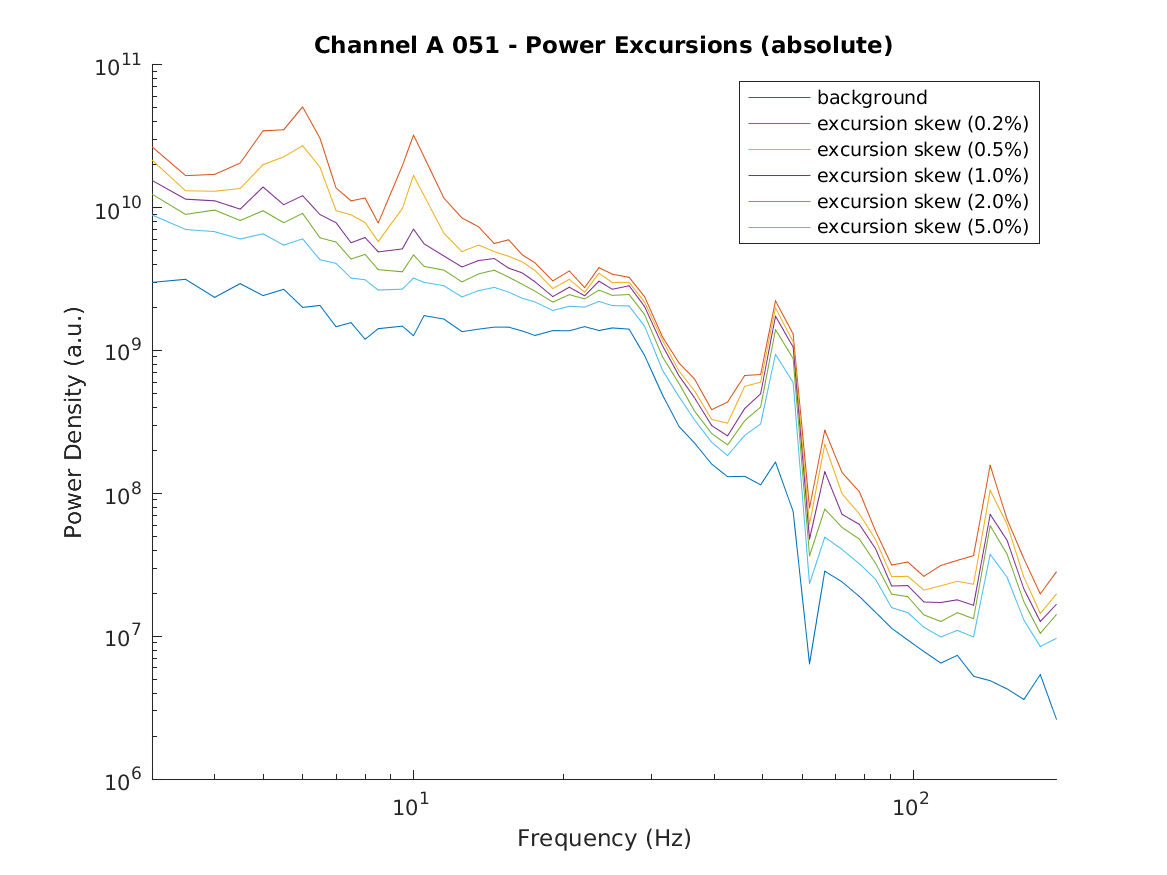
\includegraphics[width=6in]{plots/20201005/spect-burst-abs-A-051}
%
\end{center}
%
\vfill
{\tiny \input{../LICENSE.md}}
%
\clearpage
%
%
% Front matter.
%
% NOTE - Putting the overview before the TOC!
%
\pagestyle{plain}
\pagenumbering{roman}
\setcounter{page}{1}
%
% Neuroloop utilities - Library reference - Overview
% Written by Christopher Thomas.

% Dummy out chapter; this is now front-matter.
%\chapter{Overview}
\vspace*{0.75in}
{\Huge \bfseries Overview}
\vspace*{\baselineskip}
\label{sect-over}

The NeuroLoop utility library functions are divided into several categories:

\begin{itemize}
%
\item \textbf{``Core''} functions (part \ref{sect-core}) are functions
useful in a wide variety of contexts (not vendor- or application-specific).
%
\item \textbf{``Abstraction''} functions (part \ref{sect-vendor}) are
functions used to support specific hardware devices or software suites.
%
\item \textbf{``Application''} functions (part \ref{sect-apps}) are
functions used by individual application programs that are either designed
specifically to interact with that application's code or that perform
tasks specific enough to limit reusability.
%
\item Lastly, part \ref{sect-samplecode} contains sample code that may
help illustrate the ways these libraries may be used.
%
\end{itemize}

``Core'' function libraries are as follows:

\begin{itemize}
%
\item \textbf{``Processing''} functions (ch. \ref{sect-proc}) perform signal
processing operations on data series such as filtering, artifact rejection,
statistical calculations, and so forth.
%
\item \textbf{``Utility''} functions (ch. \ref{sect-util}) perform
miscellaneous operations that are not covered by the other categories.
%
\item \textbf{``I/O''} functions (ch. \ref{sect-io}) facilitate operations
for reading and writing data that aren't vendor-specific.
%
\item \textbf{``Plotting''} functions (ch. \ref{sect-plot}) render plots
of various types to files, figures, or axes. These are included as an aid
to rapid prototyping, and are used by the GUI scripts. The output is
generally not publication-ready.
%
\end{itemize}

``Abstraction'' function libraries are as follows:

\begin{itemize}
%
\item \textbf{``Field Trip''} functions (ch. \ref{sect-ft}) facilitate
interoperation with Field Trip.
%
\item \textbf{``Intan''} functions (ch. \ref{sect-intan}) facilitate the use
of datasets stored in Intan's format.
%
\item \textbf{``Vendor-Supplied Intan''} functions
(ch. \ref{sect-vend-intan}) are functions derived from vendor-supplied code
that are in turn wrapped by the functions in ch. \ref{sect-intan}.
%
\item \textbf{``Open Ephys''} functions (ch. \ref{sect-openephys})
facilitate the use of datasets stored in Open Ephys's format.
%
\end{itemize}

% FIXME - Force a page break here.
\clearpage
``Application'' library functions are as follows:

\begin{itemize}
%
\item \textbf{``Channel Tool''} functions (ch. \ref{sect-chan}) perform
operations used by the ``Channel Tool'' utility. The intention is that all
operations that are not tied to GUI implementation are packaged as library
functions for reuse outside of that application.
%
\item \textbf{``Sanity check''} functions (ch. \ref{sect-sanity}) perform
operations used by the in-house dataset ``sanity checking'' utility. These
functions encapsulate operations that are not lab-specific.
%
\end{itemize}

Relevant notes about data structures and file structures used by the
various libraries are described in their associated ``Additional Notes''
chapters.

%
% This is the end of the file.

\clearpage
%
\tableofcontents
\clearpage
%
%
% Document parts.
%
\pagestyle{plain}
\setcounter{page}{1}
\pagenumbering{arabic}
%
\part{Core Libraries}
\label{sect-core}
%
\input{nlutilref-notes-core}
%
\input{nlutilref-proc}
\input{nlutilref-util}
\input{nlutilref-plot}
\input{nlutilref-io}
%
\part{Abstraction Libraries}
\label{sect-vendor}
%
\input{nlutilref-notes-vendor}
%
\input{nlutilref-ft}
%
\input{nlutilref-intan}
\input{nlutilref-vend-intan}
%
\input{nlutilref-openephys}
%
\part{Application Libraries}
\label{sect-apps}
%
\input{nlutilref-notes-apps}
%
\input{nlutilref-chantool}
\input{nlutilref-sanity}
%
\part{Sample Code}
\label{sect-samplecode}
%
\input{nlutilref-examples}
%
%
\end{document}

%
% This is the end of the file.
